\chapter{Electroosmotic flow and advected species}

\modinfo{Directory}{Microfluidic}
\modinfo{Solvers}{\Idx{StatElecSolve}, \Idx{FlowSolve },
  \Idx{AdvectionDiffusion}, \Idx{Electrokinetics}}
\modinfo{Tools}{\Idx{ElmerGrid}, editor}
\modinfo{Dimensions}{2D}


\subsection*{Case definition}

This tutorial is an example of setting up a simulation for
(microfluidic) electroosmotic flow advecting a passive scalar
quantity. Diffusion of the species is also included. The geometry of
the system is a simple 2D microchannel with T crossing. The flow is
induced by the applied electric field and the electric double layer at
the channel walls. The analyte (species) is inserted into the system
from the left hand side inlet.

More details on the electrokinetic capabilities of Elmer are found on
the Models Manual, chapter ``Electrokinetics''.


\subsection*{Solution Procedure}

The computatonal mesh is done with \texttt{ElmerGrid} in directory
\texttt{Tcross} with the command 
%
\ttbegin
ElmerGrid 1 2 Tcross -scale 1e-5 1e-5 1e-5
\ttend
%
The scale option above is used to obtain appropriate dimensions from a
geometry template defined in nondimensional units.

The command file may be written with a text editor. The file includes
the following information. 

The mesh directory is given in the header of the command file
%
\ttbegin
Header
  Mesh DB "." "Tcross"
End
\ttend
%
The simulation block of the command file defines, eg., the case to be time
dependent (transient) with $10^{-5}$ second time steps and altogether
120 time intervals. Results from every second time step are saved into
the files \texttt{diffusion1.*}.
%
\ttbegin
Simulation
  Coordinate System = Cartesian 2D

  Simulation Type = "Transient"
  Steady State Max Iterations = 20

  Timestep Intervals = 120
  Timestep Sizes = 1e-5  
  Output Intervals = 2

  Timestepping Method = BDF
  BDF Order = 2

  Binary Output = Logical True

  Output File = "diffusion1.res"
  Post File = "diffusion1.ep"

  Output Version Numbers = Logical True
  Max Output Level = 32
End
\ttend
%
The electrostatics and electrokinetics solvers require the value of
the permittivity of vacuum. This is actually not even needed here
since the case deals with conducting media. Thus the value has been
fixed as 1.0 to avoid warnings on missing constant definitions.
%
\ttbegin
Constants
!  Permittivity Of Vacuum = 8.8542e-12  ! C\verb|^2|/Nm\verb*|^2|
  Permittivity Of Vacuum = 1.0 ! manipulation for conducting material
End
\ttend
%
The case includes only one body. The corresponding equation definitions are
found in section \texttt{Equation 1} and material parameters from
section \texttt{Material 1}.
%
\ttbegin
Body 1
  Equation = 1
  Material = 1
End
\ttend
%
All three solvers are active in this equation set. Further definitions
include, first, that the convection of the species is switched on
(besides diffusion). Then that for Navier-Stokes equations the
convective term may be left out resulting in laminar Stokes flow, and
finally that the electric field is computed by the electrostatics
rather than given by the user.
%
\ttbegin
Equation 1
  Active Solvers(3) = 1 2 3
  Convection = Computed
  NS Convect = False
  Electric Field = String "computed"
End
\ttend
%
Following are the solver definitions. Solver 1 is the electrostatics
solver. The equation is linear and thus no non-linear iterations are
needed. The equation is solved using a fast direct method UMFPack.
%
\ttbegin
Solver 1  
  Equation = "Stat Elec Solver"
  Procedure = "StatElecSolve" "StatElecSolver"
  Variable = String "Potential"
  Variable DOFs = 1

  Calculate Electric Field = True
  Calculate Electric Flux = False
  Linear System Convergence Tolerance = 1.0E-10

  Linear System Solver = Direct
  Linear System Direct Method = UMFPack 
  Linear System Preconditioning = ILU1
  Linear System Residual Output = 1

  Nonlinear System Max Iterations = 1
  Nonlinear System Convergence Tolerance = 1.0e-10
  Steady State Convergence Tolerance =  1.0E-10
End
\ttend
%
The next solver is for the Navier-Stokes equations. Here non-linear
iterations are required.
\ttbegin
Solver 2
  Equation = "Navier-Stokes"

  Linear System Convergence Tolerance = 1.0D-08
  Linear System Solver = Iterative
  Linear System Iterative Method = "BiCGStab"
  Linear System Max Iterations = 500
  Linear System Abort Not Converged = False  ! True
  Linear System Preconditioning = ILU1 
  Linear System Residual Output = 10  

  Nonlinear System Convergence Tolerance = 1.0e-6
  Nonlinear System Max Iterations = 30
  Nonlinear System Newton After Iterations = 10
  Nonlinear System Newton After Tolerance =  Real 1.0D-8
  Nonlinear System Relaxation Factor = 1.0
  Steady State Convergence Tolerance =  1.0D-03

  Stabilize = True
End
\ttend
%
The advection-diffusion equation does not affect either the
electrostatic field or the flow, thus it may be solved only after a
converged solution for the previous two equations is available. This
is achieved with the \texttt{Exec Solver} definition below. The
advected quantity is given the name Analyte.
The advection-diffusion solver uses bubble stabilization method to
avoid numerical problems associated with convection type equations.
%
\ttbegin
Solver 3
  Exec Solver = After Timestep
  Equation = "Analyte transfer"
  Procedure = "AdvectionDiffusion" "AdvectionDiffusionSolver"
  Variable = String "Analyte"
  Variable DOFs = 1

  Bubbles = True

  Linear System Convergence Tolerance = 1.0E-06
  Linear System Solver = "Iterative"
  Linear System Iterative Method = "BiCGStab"
  Linear System Max Iterations = 500
  Linear System Preconditioning = ILU2
  Linear System Residual Output = 1

  Nonlinear System Max Iterations = 1
  Nonlinear System Convergence Tolerance = 1.0e-5
  Steady State Convergence Tolerance =  1.0D-06
End
\ttend
%
The material parameters are given below.
%
\ttbegin
Material 1
  Density = 1e3  
  
  Viscosity = 1e-03

  Relative Permittivity = 1.0    !  this is actually electric conductivity

  Analyte Diffusivity = Real 1e-10 
End
\ttend
%
Finally the boundary conditions are defined. The first BC is given for
the channel walls. Here, tangential velocity (velocity components 1
and 2) is computed by the Helmholtz-Smoluchowski slip velocity
condition, which means that the velocity is computed using the
computed electric field and the electroosmotic mobility as inputs. 
%
\ttbegin
Boundary Condition 1
  Name = "channel-walls"
  Target Boundaries(2) = 4 5

  EO Mobility = Real 5e-08 

  Velocity 1 = Variable Pressure
      Real Procedure  "Electrokinetics" "helmholtz_smoluchowski1"
  Velocity 2 = Variable Pressure
      Real Procedure  "Electrokinetics" "helmholtz_smoluchowski2"
End
\ttend
%
The next BC is the inlet condition. We give a potential of 100 Volts
and define that there is no flow in $y$-direction. The analyte
concentration at the inlet is defined as a function of time using
table format. The concentration is 1.0 up until time instant $3\cdot
10^{-5}$, is zero after $4\cdot 10^{-5}$s and decreases linearly
between these two time instants.
%
\ttbegin
Boundary Condition 2
  Name = "el_A"
  Target Boundaries = 1

  Potential = 100.0

  Velocity 2 = 0.0

  Analyte = Variable Time
    Real
      0.0      1.0
      3.0e-5   1.0
      4.0e-5   0.0
      0.5      0.0
    End

End
\ttend
% 
The final two boundary conditions are for the outlets. Different
potentials for these are defined as well as a condition for velocity
component.
%
\ttbegin
Boundary Condition 3
  Name = "el_B"
  Target Boundaries = 2

  Potential = 30.0

  Velocity 1 = 0.0
End

Boundary Condition 4
  Name = "el_C"
  Target Boundaries = 3

  Potential = 0.0 

  Velocity 1 = 0.0
End
\ttend
%
After writing the command file is finished, the problem can be solved
by entering the command \texttt{ElmerSolver} on the command line. The
results can be examined with \texttt{ElmerPost}.


\subsection*{Results}

Solving the problems takes less than a minute cpu time on a PC. The
maximum and minimum concentration over the whole simulation are 1.0235
and -0.075748. The solution of this problem should be between 0 and
1. This shows that some numerical discretization errors are present in
the simulation. The errors would diminish when using smaller time steps
and also with denser mesh. Simulation results at the time
instant of 0.00025 seconds are shown in Fig.~\ref{fig:analyte_ek}.

\begin{figure}[bht]
\begin{center}
  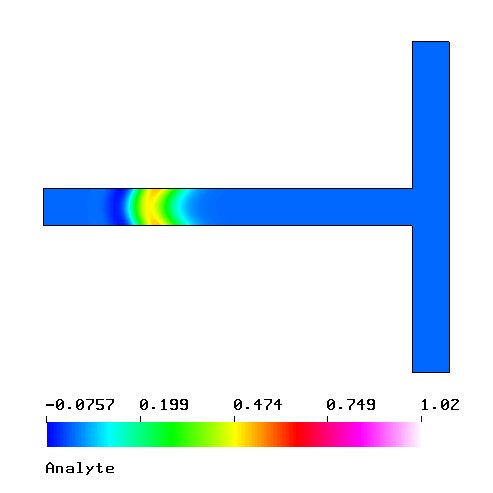
\includegraphics[height=0.55\textwidth]{analyte_tutorial.png}
\end{center}
\caption{Analyte concentration on time instant 0.00025 seconds.}
\label{fig:analyte_ek}
\end{figure}
 
The maximum value of the magnitude of the velocity in the results is
0.105 m/s.

The electric field is written into the output only component wise. The
magnitude of the field may be visualised after giving the following
commands on the ElmerPost command line (assuming one has read in all
61 time steps):
%
\ttbegin
math E(0,time(0):time(61)-1) = Electric.field.1
math E(1,time(0):time(61)-1) = Electric.field.2
math E(2,time(0):time(61)-1) = 0
math E_abs = sqrt(vdot(E,E))
\ttend
%
Now visualising the variable \texttt{E\_abs} reveals that the electric
field magnitude is between 2453 and $2.18\cdot10^6$.


\subsection*{Notes}

When checking the simulation results the user will notice that the
electric potential does not change in time and that the flow reaches
steady-state within a few time steps. This is quite clear also from the
problem setup: the electric field is due to unvarying potential with
constant material parameters. Also the flow in microchannels is
usually laminar.

Thus the most efficient way to simulate the current case would be to
compute first the steady-state solution for the electrokinetic flow
and use the steady flow to advect the analyte. This would be done by
running two separate simulations; resolve first the steady flow,
and to use this flow solution as restart for the advection-diffusion
equation.



\hfill